\documentclass[11pt]{amsart}
\usepackage{geometry}                % See geometry.pdf to learn the layout options. There are lots.
\geometry{a4paper}                   % ... or a4paper or a5paper or ... 
%\geometry{landscape}                % Activate for for rotated page geometry
\usepackage[parfill]{parskip}    % Activate to begin paragraphs with an empty line rather than an indent
\usepackage{graphicx}
\usepackage{amssymb}
\usepackage{epstopdf}
\usepackage{caption}
\usepackage{subcaption}

\DeclareGraphicsRule{.tif}{png}{.png}{`convert #1 `dirname #1`/`basename #1 .tif`.png}

\title{The Wide Role of Informatics at Universities}
\author{E Di Nitto \and S Eisenbach \and I Garcia, E Gr\"{o}ller \and C Sadler}
%\date{}                                           % Activate to display a given date or no date

\begin{document}
\maketitle
\section{Introduction}

In the 1970s with the advent of the personal computer we entered into the Digital or Information Age. However it has only been in this century with the ubiquity of the internet, the smartphone, and the internet of things that digital has become truly pervasive. How do universities respond to this massive change? Informatics Europe established in 2018 a new working group to investigate what universities are doing to ensure that non-informatics teaching and research is informed by best practice in Informatics.

To better understand the state of affairs on this topic and discover best practices at European Universities, the working group conducted an online survey. We invited heads and members of Informatics/Computer Science/IT Departments (Schools, Faculties, Institutes) to complete a questionnaire in autumn 2018. The request to fill out our survey was sent to all Informatics Europe members and it was also publicly available from the Informatics Europe website.  For the location of the respondents see Figure~\ref{fig:mapandmembers}.  Forty eight universities from nineteen countries filled it out (see Appendix~\ref{apx:names}).

\begin{figure}[h]
\centering
\begin{subfigure}{.5\textwidth}
  \centering
  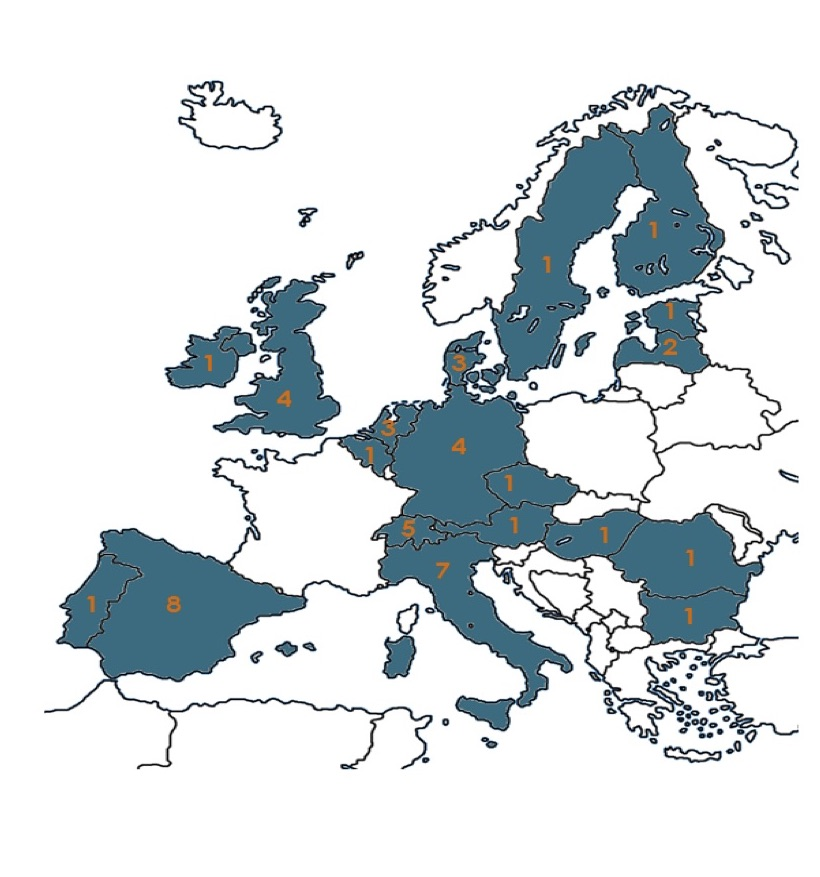
\includegraphics[width=\linewidth]{charts/map.jpg}
  \caption{Countries}
  \label{fig:map}
\end{subfigure}%
\begin{subfigure}{.5\textwidth}
  \centering
  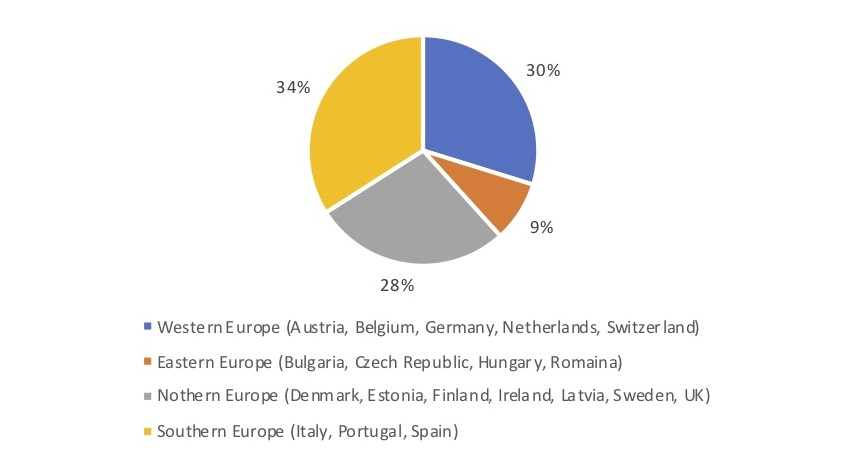
\includegraphics[width=1.5\linewidth]{charts/regions.jpg}
   \caption{Regions}
  \label{fig:members}
\end{subfigure}
\caption{Location of Respondents}
\label{fig:mapandmembers}
\end{figure}

Our survey was wide ranging. We wanted to understand how universities valued interdisciplinary research, about teaching Informatics to non-specialist students, what happens in practice with hiring and supporting interdisciplinary academics, and what structures are in place to support interdisciplinary work. We chose to examine Data Science's impact in detail, given its importance and newness. For the actual survey questions see Appendix~\ref{apx:survey}. 

Although how Informatics (also called Computer Science or Computing) should position itself in a university is a political decision, in many universities what happens has arisen organically rather than strategically. There are a wide range of models with the extremes ranging from primarily being a service department to being primarily a research area that is isolated from other departments.

\section{research}

Universities are normally structured into disciplines which foster disciplinary research. However, the ubiquity of Informatics in our culture has led to pressures for research that is interdisciplinary. Pressures in favour of such research comes from academics themselves, student interests, external funding sources, and sometimes from university leadership. The 
following subsections discuss the answers obtained for each specific
question.

\subsection{Desirability of interdisciplinary research}

\begin{figure}[h]
\centering
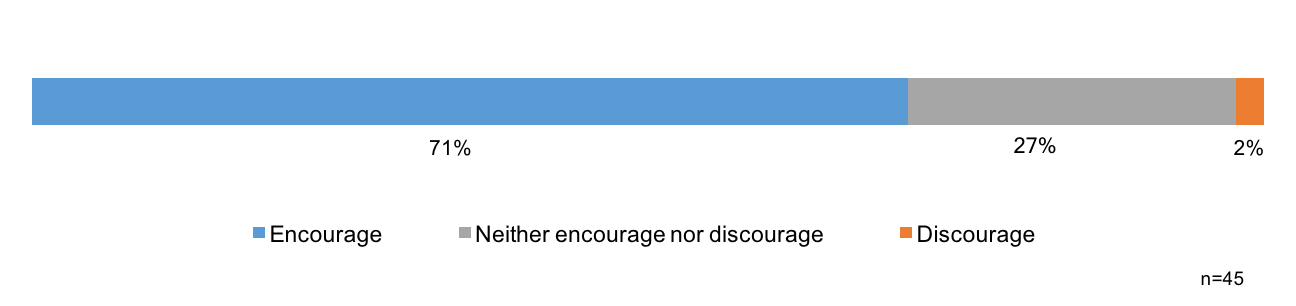
\includegraphics[width = \linewidth]{charts/1a.png}
\caption{What is the University attitude towards Interdisciplinary research?}
\label{sect1:Uattitude}
\end{figure}

The first part of the survey questioned respondents on university attitudes and actions in respect of interdisciplinary research.\footnote{The survey does not differentiate between interdisciplinary work in general and that with an Informatics component. Given who answered the questionnaire, one can assume that Informatics is included} A large majority (71\%) claimed that their university encouraged interdisciplinary research when compared with single discipline research (see Figure~\ref{sect1:Uattitude}). This seems to imply that universities favour interdisciplinary research over single discipline research.  However, several respondents indicated that their encouragement was largely `theoretical' and accompanied by little, if any, funding. Some respondents said that much of the interdisciplinary work at their institution occurred between departments other than Informatics. Only one respondent indicated that their university actually discouraged interdisciplinary research although others mentioned that their departments were judged, usually nationally, against discipline-specific criteria.

\subsection{Department attitude towards Interdisciplinary research}


\begin{figure}[h]
\centering
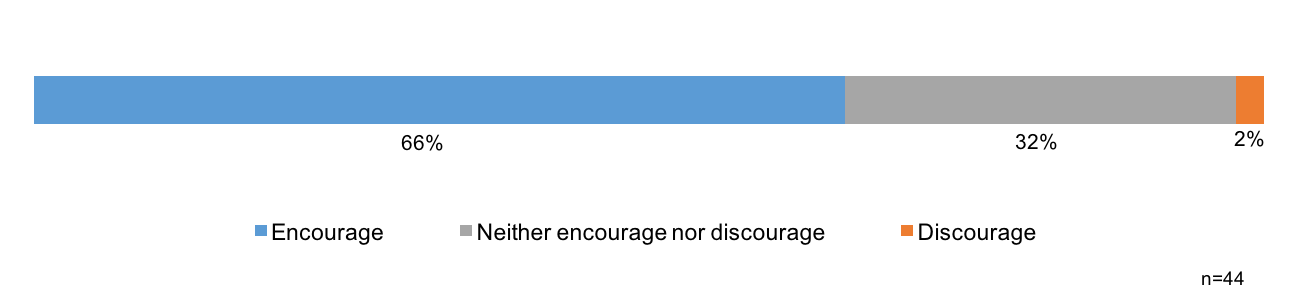
\includegraphics[width = \linewidth]{charts/1b.png}
\caption{What is the Department attitude towards interdisciplinary research?}
\label{sect1:Dattitude}
\end{figure}

With the same question directed at Informatics Departments rather than the whole university (see Figure~\ref{sect1:Dattitude}), two thirds of respondents still claimed that interdisciplinary research was favoured over single discipline topics. However, similar comments are made about encouragement being in principle rather than in practice and about being judged on discipline-specific criteria.

\subsection{University support}

\begin{figure}[h]
\centering
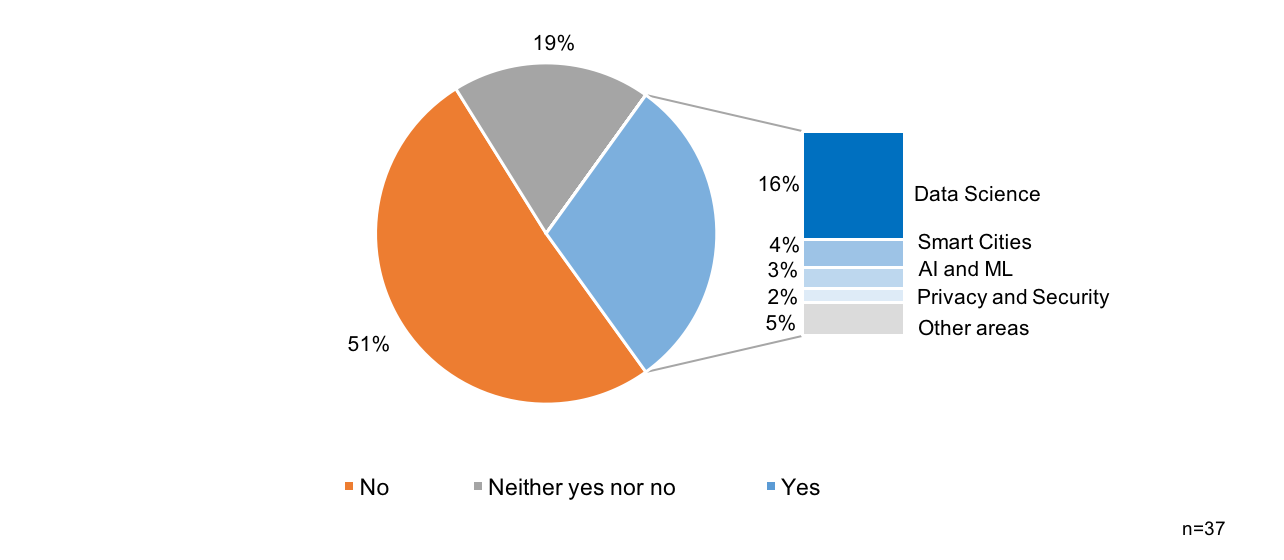
\includegraphics[width = \linewidth]{charts/1c.png}
\caption{Are there interdisciplinary areas of research where your university
could enter but aren't due to lack of university support?}
\label{sect1:support}
\end{figure}

However, just over half (51\%) of the respondents recorded (see Figure~\ref{sect1:support}) that their university supported all areas of interdisciplinary research which required  support. Others (30\%) mentioned a variety of potential informatics areas where university support for interdisciplinary research was lacking. Others talked of the need for strategic planning to direct interdisciplinary efforts or of the need to focus given the wide range of potential opportunities.

\subsection {Additional support}

\begin{figure}[h]
\centering
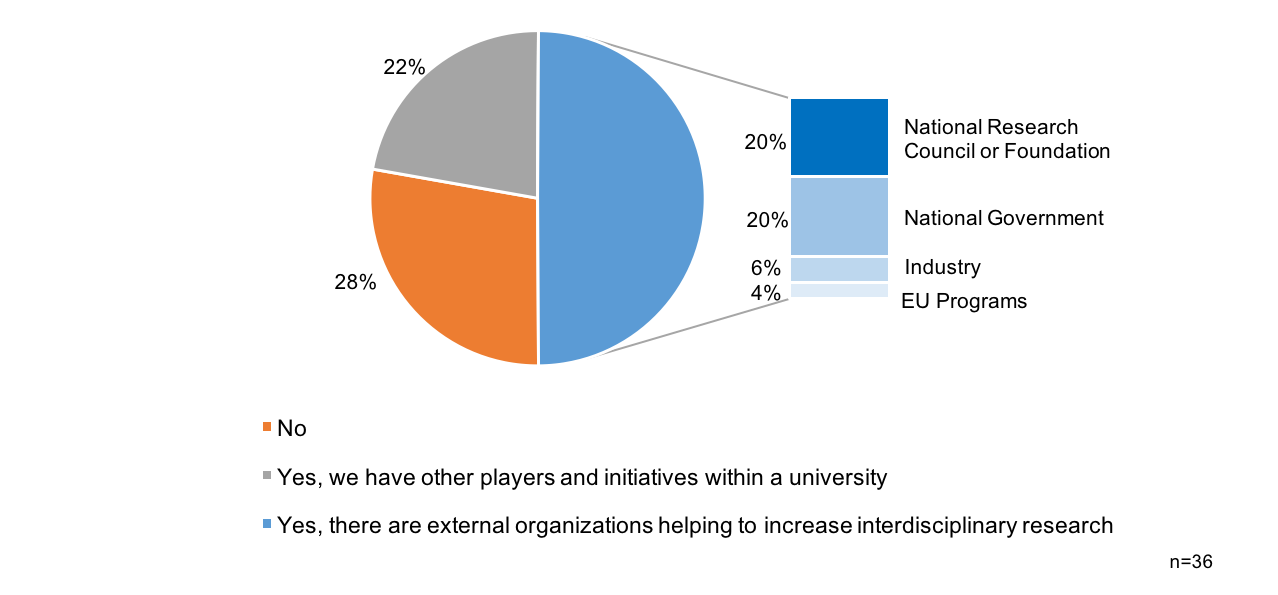
\includegraphics[width = \linewidth]{charts/1d.png}
\caption
{Are there other players who have helped increase the
interdisciplinary research in your university?}
\label{sect1:additional}
\end{figure}

When asked about external support for interdisciplinary research directed towards their university (see Figure~\ref{sect1:additional}), 50\% of the respondents responded positively with 40\% stating that national public funding sources had helped to increase interdisciplinary research. A further 22\% mainly discussed specific formal or informal arrangements between their department and others in their institution.

\subsection{Final thoughts}

Respondents were asked to make some more general comments. Not all respondents were especially supportive of interdisciplinary research per se. It was noted that, because some funding streams demand interdisciplinarity, it is possible that `artificial collaborations' were formed that attracted the funds but did not make good use of the capabilities of the researchers. Frequently interdisciplinary projects are focussed on how information technology can serve the other discipline so the progress made and any breakthroughs that occur advance the other discipline but have no impact on the development of Informatics. One respondent suggested that the excitement and interest in supporting interdisciplinary projects could make it likely that lower quality proposal were accepted (compared with single discipline ones).

Respondents with more positive attitudes towards interdisciplinary research were often nevertheless concerned about its development mainly owing to limited funding, low esteem compared with discipline-specific research or lack of strategic direction.


\section{teaching}

Inmaculada Garcia Fernandez

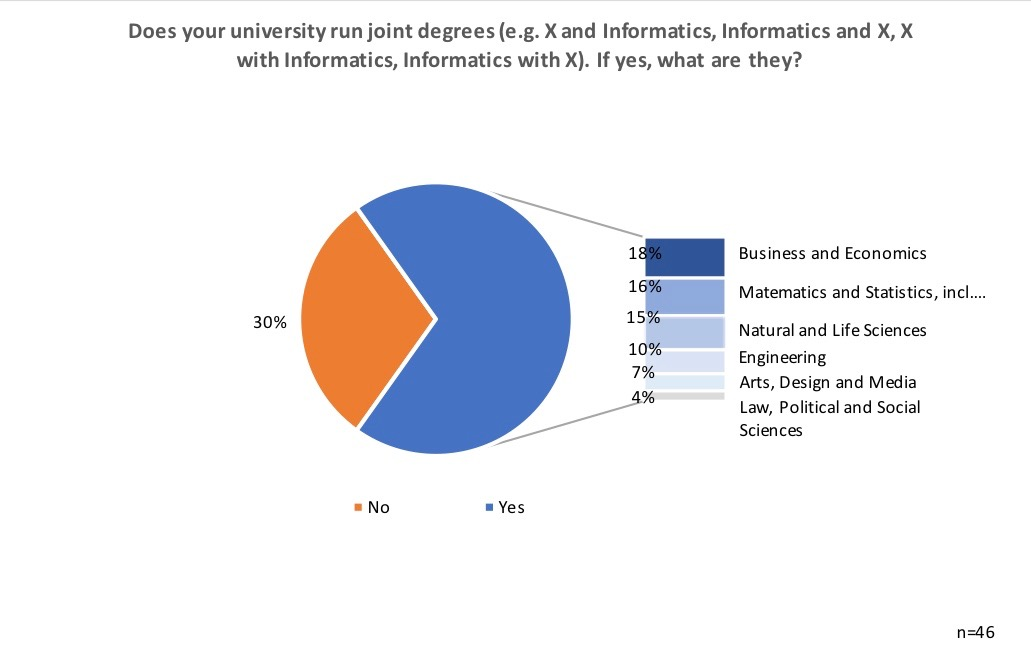
\includegraphics[width = \linewidth]{charts/2a.jpg}

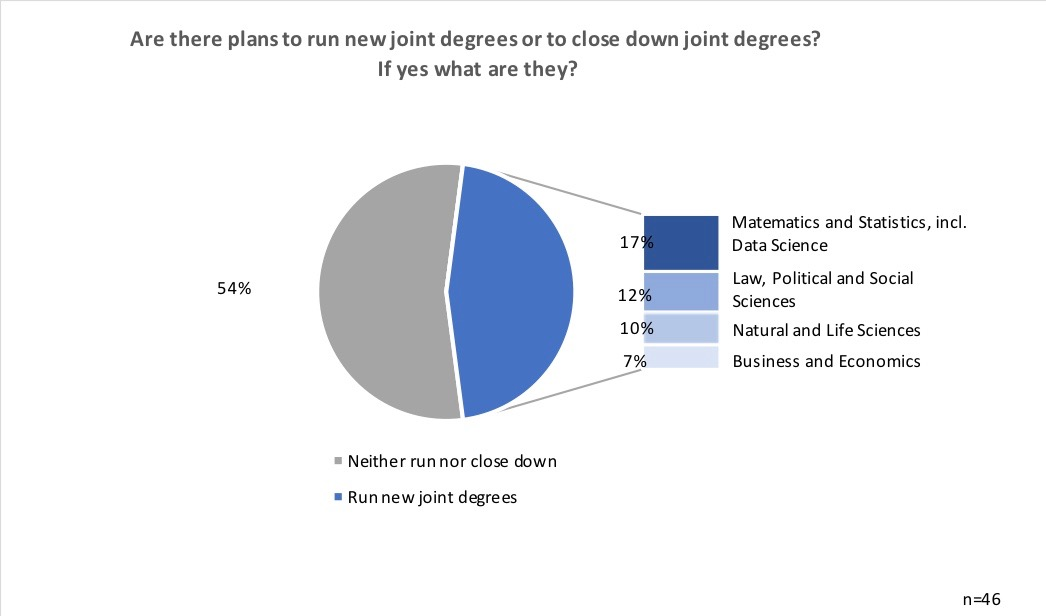
\includegraphics[width = \linewidth]{charts/2b.jpg}

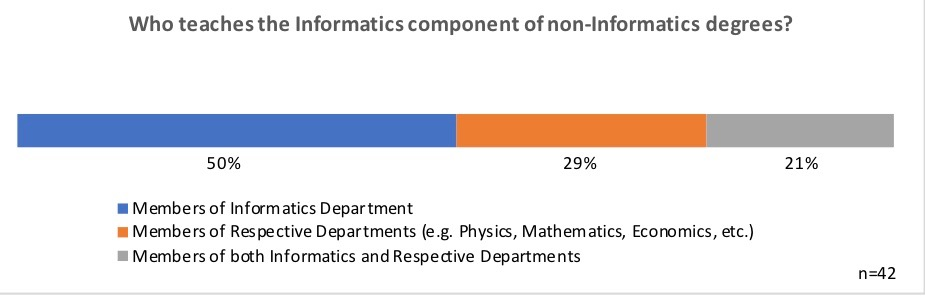
\includegraphics[width = \linewidth]{charts/2c.jpg}

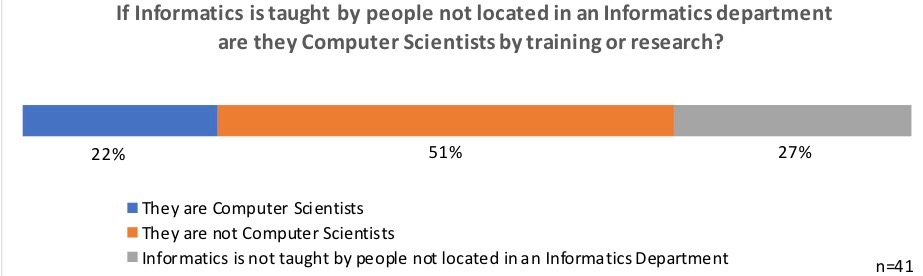
\includegraphics[width = \linewidth]{charts/2d.jpg}

\section{people}

Elisabetta Di Nitto

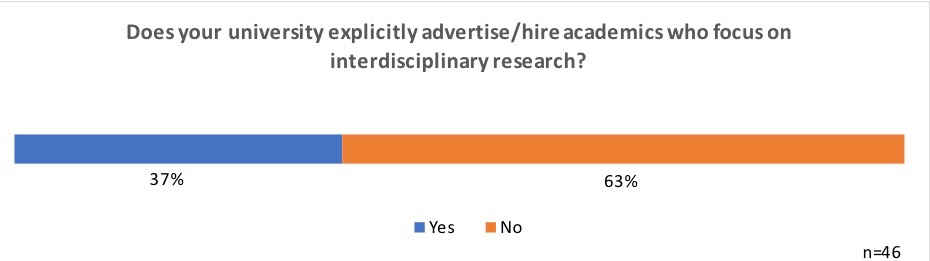
\includegraphics[width = \linewidth]{charts/3a.jpg}


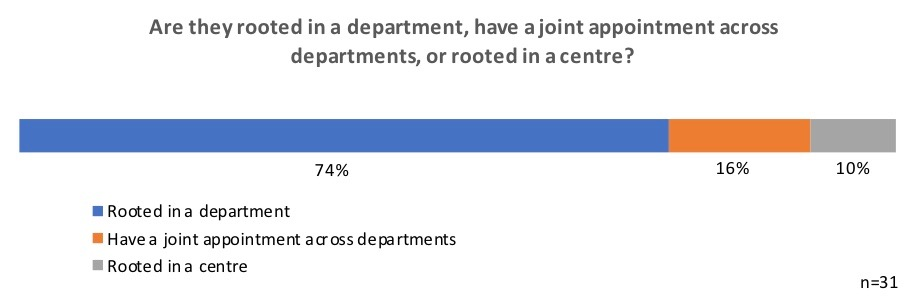
\includegraphics[width = \linewidth]{charts/3b.jpg}


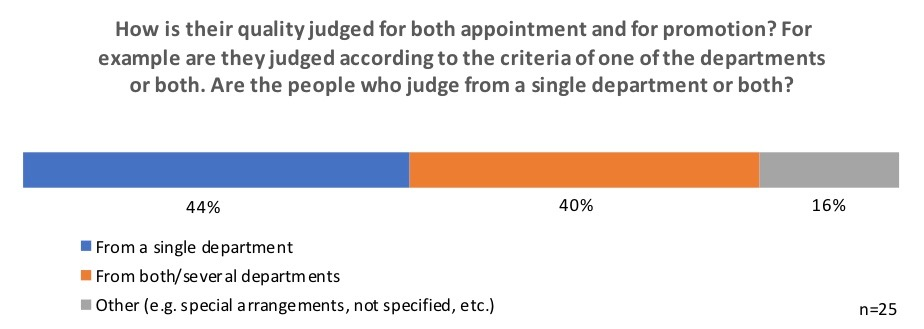
\includegraphics[width = \linewidth]{charts/3c.jpg}


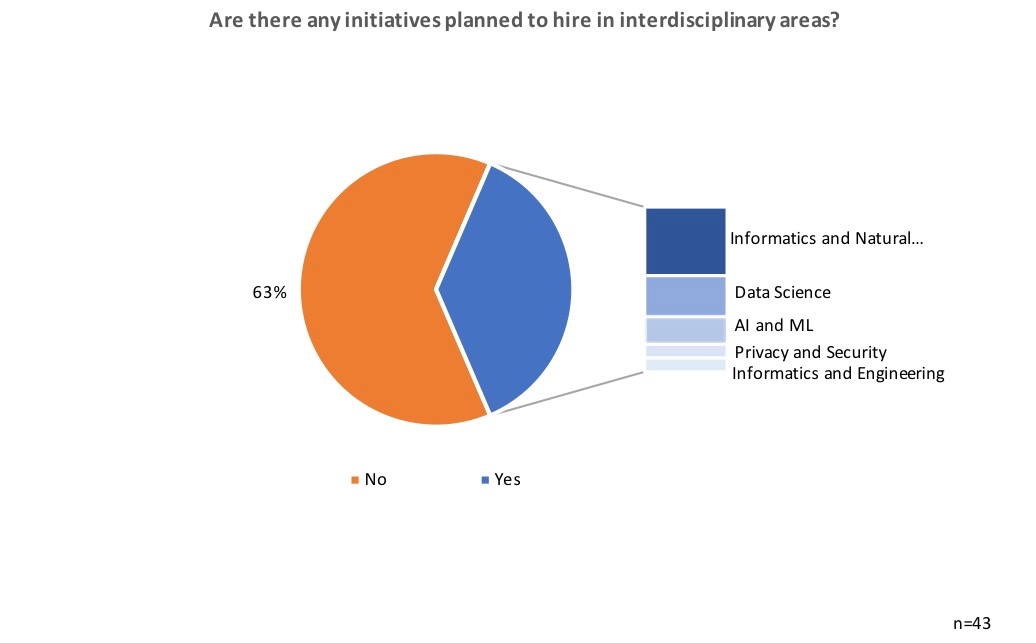
\includegraphics[width = \linewidth]{charts/3d.jpg}

\section{Data Science}

The progressing digitalisation of all aspects of human activities has tremendously increased the available data and their complexity with respect to volume, veracity, velocity, and variety. Terms like big and smart data have been coined to point towards a fourth way of scientific knowledge generation. Following experimental sciences, theoretical sciences and computational sciences, the rather new field of Data Science has been rapidly emerging in recent years. Data science extracts knowledge from data in a generalisable way. It explores, abstracts, and communicates intricate systems through simplified models derived from data. Based on large and rapidly growing data repositories, Artificial Intelligence, machine and deep learning, with subareas like convolutional neural networks (CNNs), have exploded in scientific research and public attention. The academic educational system is only beginning to adjust their curricula to the appertaining challenges. A rapid increase in the analytics and Data Science job market is predicted, where the data scientists will have to master a very diverse skill set. Examples include the use of programmable tools to prepare and preprocess the data, generating engaging visualisations, estimating the confidence of the generated results, and automating the analysis process to increase repeatability. Learning Data Science involves very many miscellaneous fields like: mathematical and computer science foundations, statistics, programming, artificial intelligence and machine learning, text mining with natural language processing, visualisation, big and smart data mining and management, data ingestion and wrangling, applying and integrated use of various toolboxes. Informatics is a key basis and enabling technology in many of these subareas. The rapid evolution of the field of Data Science and its inherent very large diversity concerning technological approaches and application areas, make the specification, shaping, and localisation of Data Science curricula especially challenging. The 
following subsections discuss the answers obtained for each specific
question.

\subsection{Data Science's Home Department}

Data Science is located in about 46\% of cases at the Informatics departments (see Figure~\ref{sect4:discipline}). In 30\% of the cases Data Science is jointly handled by the Informatics and Mathematics/Statistics departments. Even more than two departments are jointly organising Data Science activities in 13\% of the cases. Only in 7\% of the cases a single department other than Informatics (e.g., Statistics, Economics, Mathematics) is the main responsible unit. This distribution indicates the central role of Informatics in the developing field of Data Science. Data science is happening in almost all disciplines, but the highest concentration of expertise and courses seem to be in the Informatics and Statistics departments. Sometimes Data Science and Artificial Intelligence are seen as cross-sectional disciplines, which are governed by groups of interested departments (from mathematics and logic to sociology and philosophy). The economic and business departments were also mentioned several times as participating together with Informatics and mathematics in Data Science activities. Examples of other single department set-ups have been given, like Bio-nano Sciences, Economics Studies, and Statistics.

\begin{figure}[h]
\centering
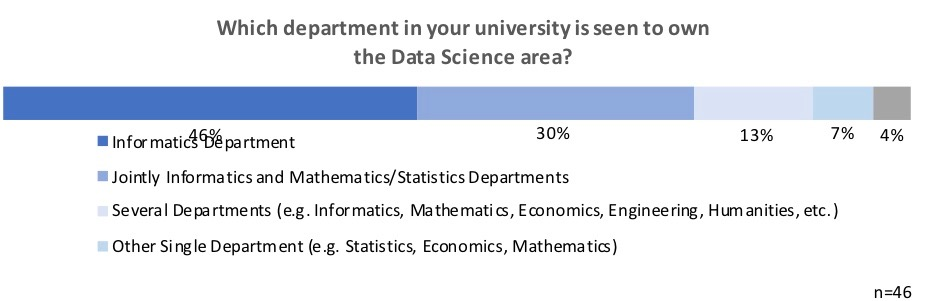
\includegraphics[width = \linewidth]{charts/4a.jpg}
\caption{Data science is part of what discipline?}
\label{sect4:discipline}
\end{figure}

\subsection{Perception of Informatics}

A large majority of 61\% of respondents indicated that the rise of Data Science has changed the perception of Informatics in the respective university (see Figure~\ref{sect4:}). Ethics and other social science aspects are considered to be increasing in relevance. There are initiatives to develop introductory courses on digital literacy and skills in all study programs. The importance of information technology is considered to be increasing beyond computational thinking to cover topics like Data Science and Machine Learning. Informatics is considered to be the main knowledge centre in the digital transformation of society and many initiatives are under way that are changing how Informatics is perceived. A growing number of non-informatics departments are asking Informatics departments to teach Data Science courses. Also, a tendency towards interdisciplinary curricula is observable (like a bridge to Statistics and Economics). At many places Informatics is recognised as an integrated part of the transformative processes currently underway. The increased relevance of Informatics is reflected in higher funding and a surge of interest in Data Science studies by potential (Informatics) students.

\begin{figure}[h]
\centering
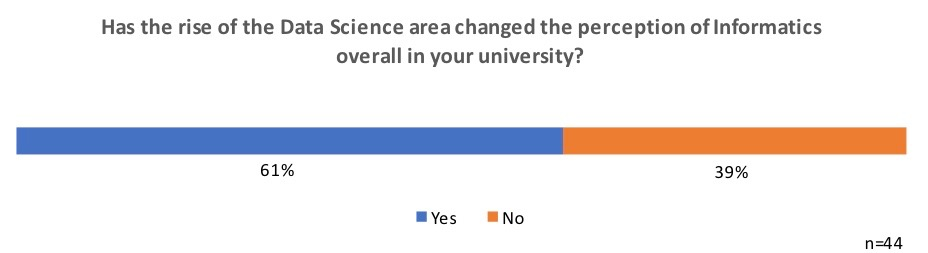
\includegraphics[width = \linewidth]{charts/4b.jpg}
\caption{Has the perception of Informatics changed with the rise of Data Science?}
\label{sect4:}
\end{figure}

\subsection{Current Arrangements at Universities}

The initiative on digital skills programs coming from the top university level beyond the Informatics department might be positive in supporting implementation acceptance. At most places the university upper levels consider the scientific and societal impact of Data Science and Artificial Intelligence rather in the (external) application domains, although an increase in Informatics students is recognisable. The early awareness of Data Science and Machine Learning as areas of rapidly increasing importance is considered crucial. Due to inertial forces (especially at larger universities), however, sometimes active strategies from the top university level is lagging, though bottom up approaches might compensate for this. As in analogous situations in the past, Informatics is struggling to be viewed only as a service department to help other domains in solving their Data Science problems. This is similar to previous interdisciplinary approaches (e.g., multimedia, computer graphics, animation) where Informatics is used as a tool, but gradually also as a research partner on an equal footing. The surge in interest in Data Science is accompanied by larger resource flows. The uncertainty about where to locate the Data Science activities might lead to the simultaneous development of several research groups at one university. This decentralised approach might allow the different departments to grow and manage their own Data Science groups with discriminative strengths. The quickly amplified interest in Data Science is primarily considered an opportunity, where it is challenging to follow and sustain all parallel activities. Currently the interest in Data Science, Machine Learning, and Artificial Intelligence is so large that this might overshadow all other areas of computer Informatics. Too imbalanced funding opportunities and student flows should be avoided to provide a well-adjusted portfolio of competences to the society and economy.

\subsection{Final Thoughts}

The interest and popularity of Data Science and Artificial Intelligence has dramatically risen in the last 10-20 years. These technologies have the potential to be driving and enabling technologies for the rapidly unfolding digital transformation of society. The very fast developments lead to many daunting challenges, e.g., concerning privacy, security, bias, reliability, robustness, legal and ethical implications. It is not yet clear where Data Science should be anchored, e.g., in the Informatics department, multi-department units, application domains, also. Due to the developmental speed, established organisations like universities are struggling to swiftly adjust their organisational structures and educational portfolios, where long term changes have yet to be implemented. For some experts in potential applications fields Data Science and Artificial Intelligence might be perceived as a hype that will cool down eventually. Despite this, most experts see the pervasive utility of informatics tools for their research area. The data scientist as a profession will be much more heterogeneous in the required skill set as compared to other interdisciplinary approaches, like Business Informatics, Bio-Informatics, or Medical Informatics, which basically involve two disciplines each. Considering the wide array of concerned fields, the data scientist will have a deep knowledge in just one or a few specialties and have a broad (and shallow) knowledge of the many other concerned areas. Data science encompasses a mixture of multidisciplinary skills ranging from mathematics/statistics, programming/databases, domain knowledge/soft skills, communication and visualisation. The fluidity of the development and the breadth of the area will transfer to Data Science groups, centres, and curricula with largely varying specialisations. It seems very likely that Informatics will play a key role in all these developments, where we should pro-actively use the many emerging opportunities.

\section{structure}

Creating actual rather than virtual interdisciplinary centres is likely to improve the chances of interdisciplinary research and teaching lasting. The following subsections discuss the answers obtained for each specific question.


\subsection{Interdisciplinary centres}

\begin{figure}[h]
\centering
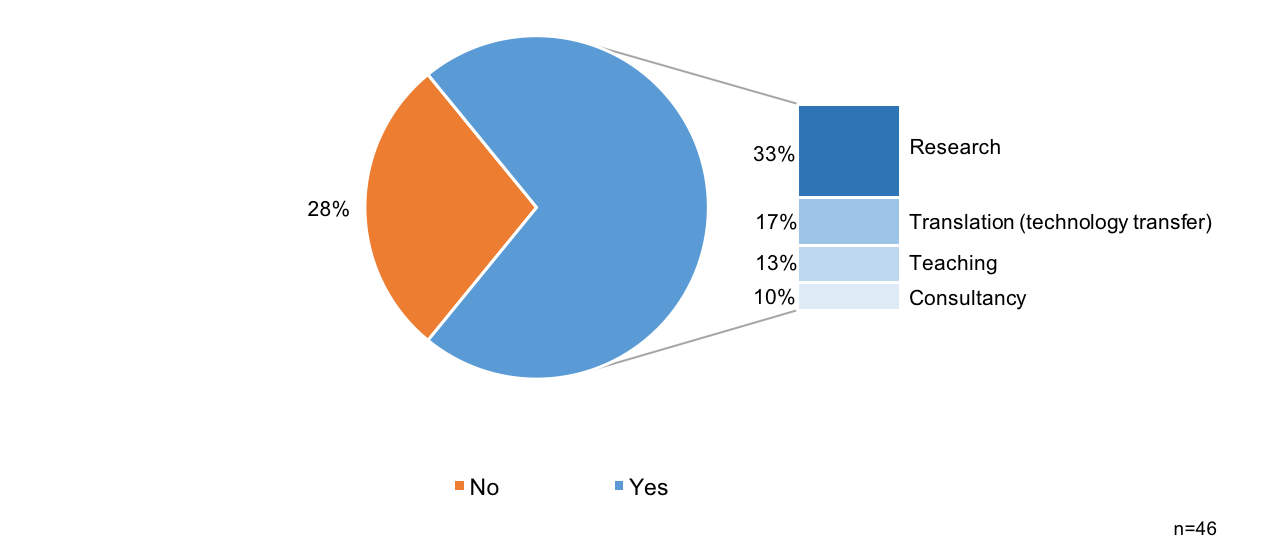
\includegraphics[width = \linewidth]{charts/5a.png}
\caption{What are the interdisciplinary centres?}
\label{sect5:centres}
\end{figure}

28\% of respondents say their university does not have real interdisciplinary centres (see Figure~\ref{sect5:centres}). Of those who commented on why the lack of centres only one actually replied that their management was averse to setting up additional administrative structures. The rest just said there were informal groupings, but nothing officially supported. 46\% of all of the interdisciplinary centres are set up primarily for research and only 18\% for teaching. The rest are primarily involved with industry.

There are a broad range of centres in the different universities -- clearly what expertise is in a university and what the structure of the different departments/schools/faculties impacts which centres are set up in addition to the existing primary structures. The most common centres mentioned with a significant Informatics component are in Computational Science, Data Science,  Life Science, Digital Society, Energy, and Security.   There were also more than one university with the following centres: Biomedical Engineering, Environment/Climate,  Medical Imaging, and  Complex Systems. There are a wide range of centres which only mentioned at one university: Health,  FinTech, Digital Humanities, Robotic Surgery, Cognitive Ageing, Bioinformatics, and Geoinformatics, 
 


\subsection{Purpose of interdisiciplinary centres}

\begin{figure}[h]
\centering
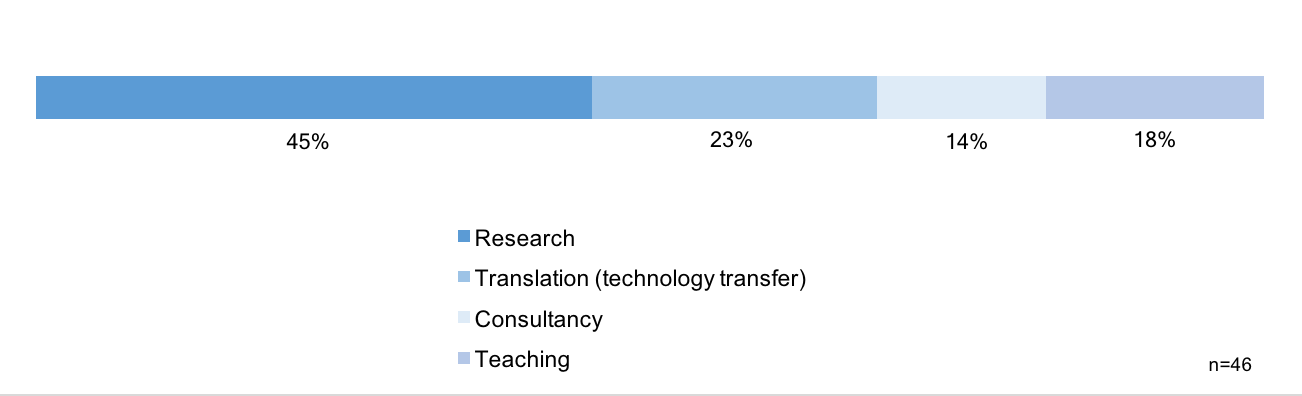
\includegraphics[width = \linewidth]{charts/5b.png}
\caption{Why were the centres created?}
\label{sect5:reasons}
\end{figure}

45\% of all of the interdisciplinary centres are set up primarily for research and only 18\% for teaching (see Figure~\ref{sect5:reasons}). The rest are primarily involved with industry collaboration or consultancy.

\subsection{ Ownership of interdisciplinary centres}

\begin{figure}[h]
\centering
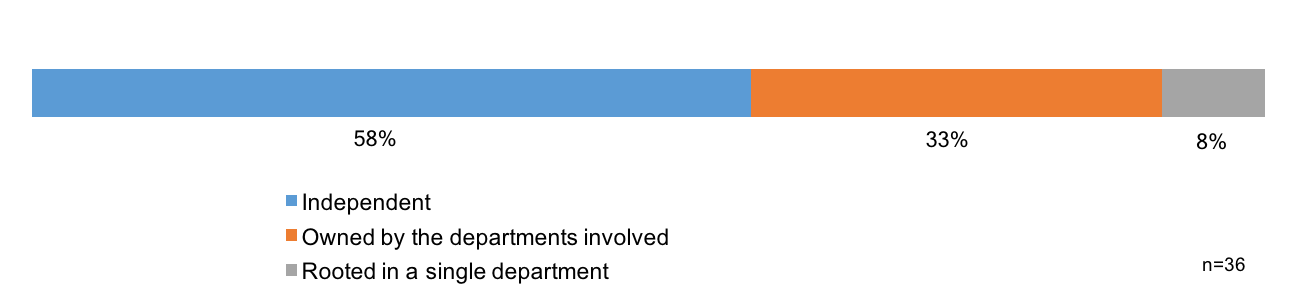
\includegraphics[width = \linewidth]{charts/5c.png}
\caption{Which entity control the interdisciplinary centres?}
\label{sect5:owners}
\end{figure}

Of the 36 respondents, 21 (or 58\%) are independent entities within their university, 12 (or 1/3) are co-owned by the departments that are involved and the rest have a single department that owns them (see Figure~\ref{sect5:owners}). It is surprising that so many are separate entities as this means if they are not self-funding money will be an issue.

\subsection{ Location of interdisciplinary centres}

\begin{figure}[h]
\centering
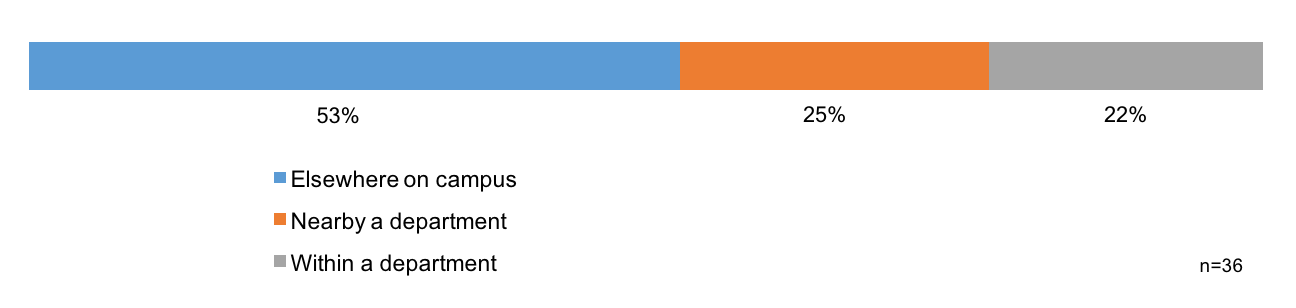
\includegraphics[width = \linewidth]{charts/5d.png}
\caption{ Where are the centres located?}
\label{sect5:locations}
\end{figure}

More than half of the respondents report that the centres they are reporting on are located `elsewhere' on campus (see Figure~\ref{sect5:locations}). although a significant minority described the centres as `virtual' implying that they actually had no physical location. One contributor distinguished between a large centre that had its own space, and smaller ones that were embedded in departments. Others spoke of large buildings that accommodated many different groups such that a nearby centre may not be associated with a department.

\subsection{Funding of interdisciplinary centres}

\begin{figure}[h]
\centering
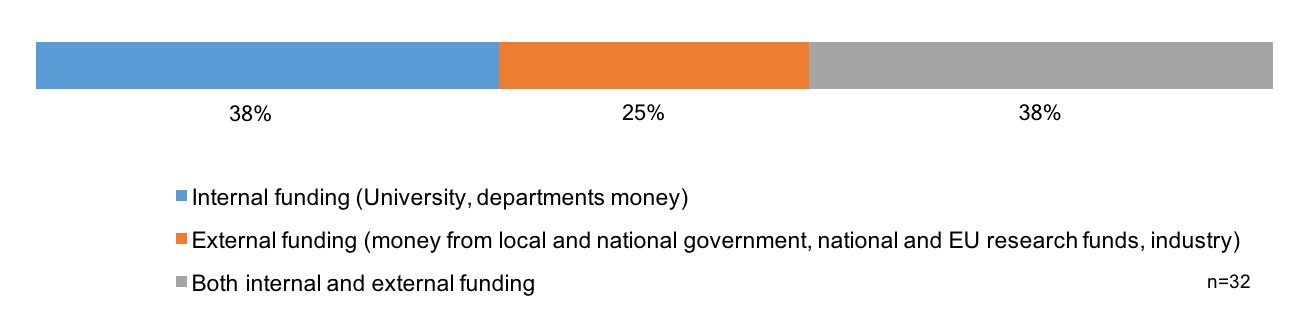
\includegraphics[width = \linewidth]{charts/5e.png}
\caption{Who funds interdisciplinary centres?}
\label{sect5:funding}
\end{figure}

Only 25\% of the interdisciplinary centres reported on are funded entirely externally, the funding of the rest being equally split between entirely internal and mixed sources of funding (see Figure~\ref{sect5:funding}). In the majority of cases where funding is entirely internal, the bulk of the actual cash seems to come from central funds with departments providing resources `in kind'. Frequently, time-limits are expressed (five and six years are mentioned) after which the centre is expected to be self-financing. For the universities that reported on (entirely or partially) external funding, in many cases only government and EU programmes were explicitly cited as sources of funds.

\subsection{Planning for changing interdisciplinary centres}

\begin{figure}[h]
\centering
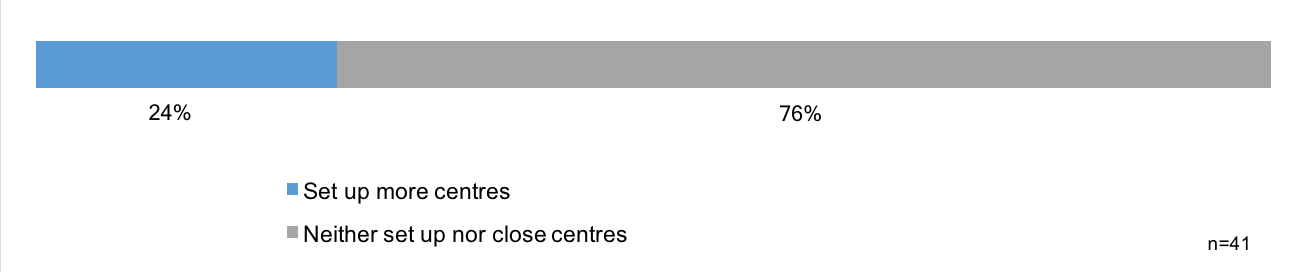
\includegraphics[width = \linewidth]{charts/5f.png}
\caption{Are there changes planned for setting up or closing centres?}
\label{sect5:changes}
\end{figure}

A quarter of respondents report on plans to set up new centres (see Figure~\ref{sect5:changes}). Some describe a notion of continuous evolution of interdisciplinary work. Only AI was explicitly mentioned as a target for the development of new centres. Other respondents, although not explicitly planning a new centre, mention the issue of the periodic review of existing centres citing various options including merging centres and/or creating new centres.  

\subsection{Drivers for new activities}

\begin{figure}[h]
\centering
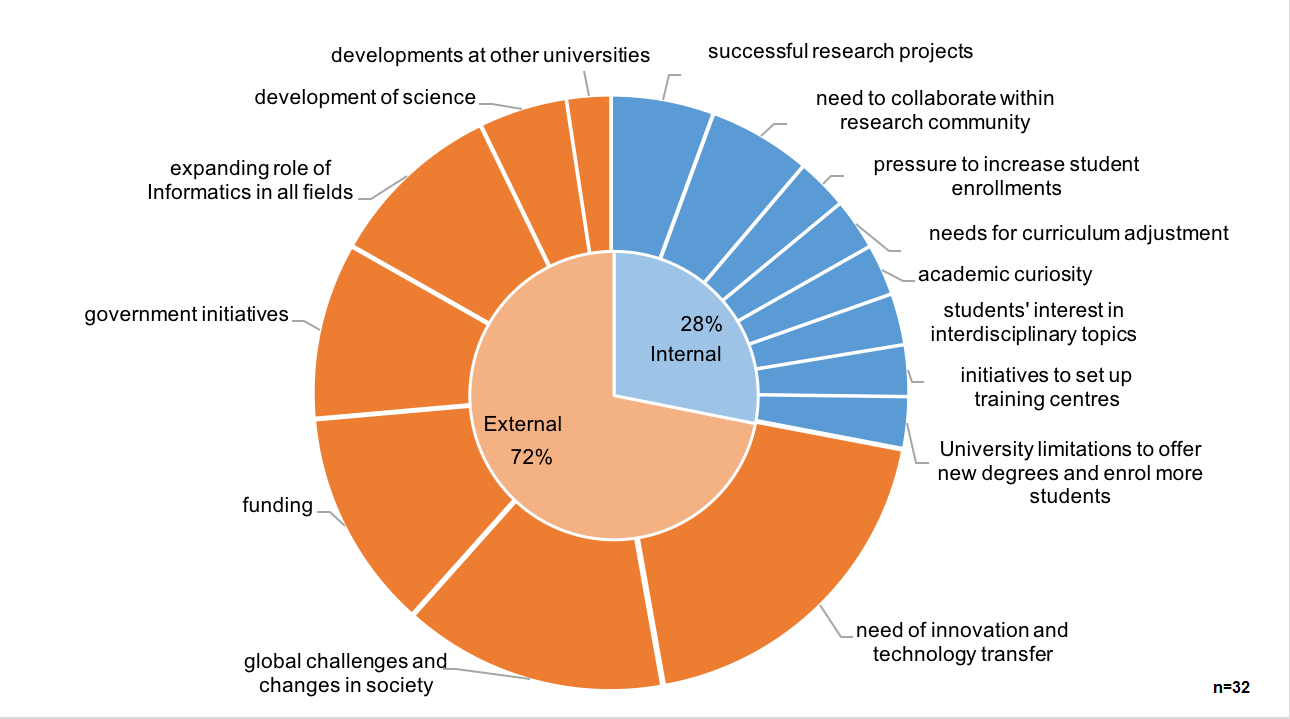
\includegraphics[width = \linewidth]{charts/5g.png}
\caption{What are the drivers for new centres?}
\label{sect5:drivers}
\end{figure}
                                                                                                                    
Nearly one third of respondents reported on internal drivers and pressures bearing on innovative activity (see Figure~\ref{sect5:drivers}). Amongst the drivers, academic curiosity of staff and students was cited alongside a need for research collaboration. Pressures included demands to increase students enrolment, to modify the curriculum and university initiatives to set up a centre. One university also mentioned limitations of student numbers and limitations on joint degrees that inhibited their development goals.

The other respondents addressed external drivers and pressures. The most significant cited pressure concerned the societal influence of globalisation together with an associated driver on universities to promote innovation and  technology transfer (47\%).  The next most significant pressure is the search for funding driven by government initiatives (30\%) whilst other respondents observed the expanding role of Informatics in other disciplines and the pressure on Informatics departments to support these disciplines (20\%). Finally, one respondent mentioned competition between universities as an external pressure.

\subsection{Support for interdisciplinary work}

\begin{figure}[h]
\centering
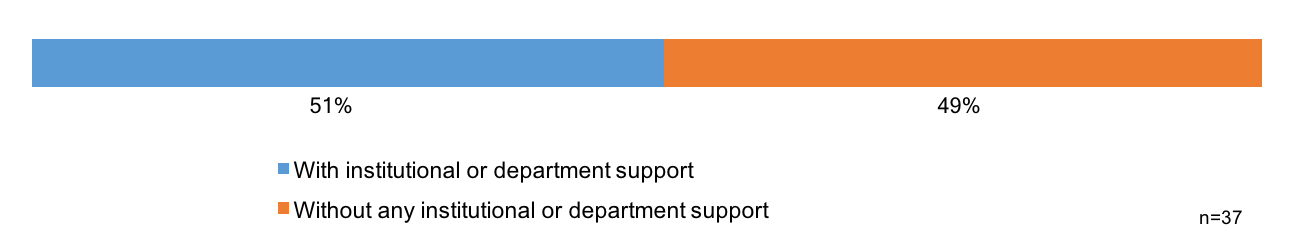
\includegraphics[width = \linewidth]{charts/5h.png}
\caption{How much support is provided for interdisciplinary work?}
\label{sect5:support}
\end{figure}

Respondents were evenly split over this question (see Figure~\ref{sect5:support}) although several of those who claimed institutional support were rather equivocal - "I would guess so" and ``Some departments \ldots ''. Respondents who reported no institutional support divided into those who stipulated some form of external support and those who did it ``as a hobby'' (~25\%).

\subsection{Strategic vision }
\begin{figure}[h]
\centering
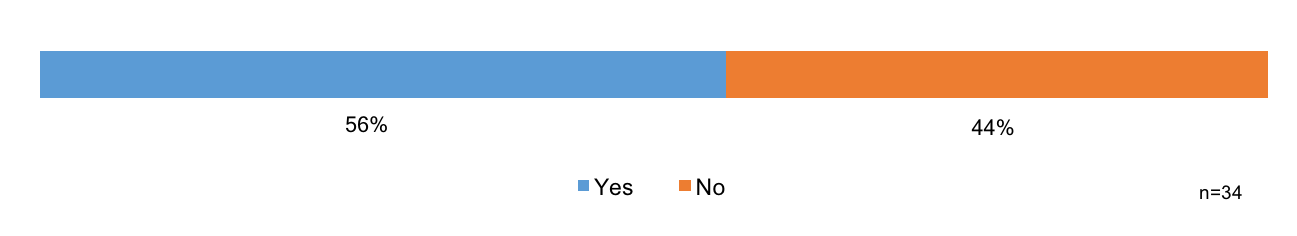
\includegraphics[width = \linewidth]{charts/5i.png}
\caption{Interdisciplinary hirings}
\label{sect5:strategy}
\end{figure}

More than half of the respondents reported on centres created from strategic initiatives (see Figure~\ref{sect5:strategy}). Many of these were oriented towards Informatics themes (FinTech, Crypto-currencies, Data Science) but several other types of centre were mentioned (Learning and Education, Cultural Heritage, Sustainability and Energy).

\subsection{Official strategic vision}
\begin{figure}[h]
\centering
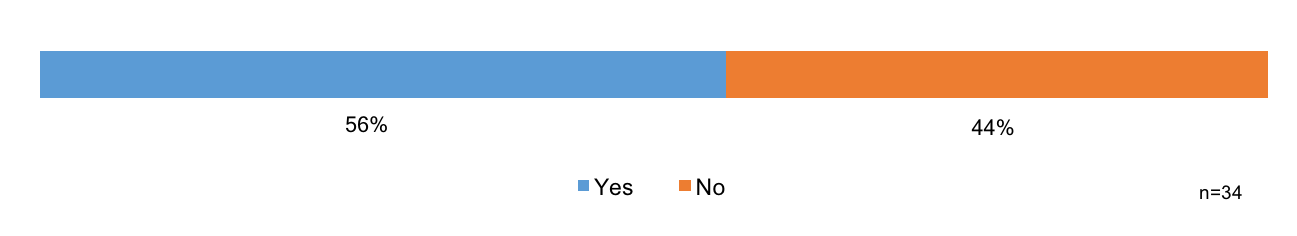
\includegraphics[width = \linewidth]{charts/5i.png}
\caption{Is there an official strategy to widen the role of Informatics?}
\label{sect5:official}
\end{figure}

Respondents were exactly split on this question (see Figure~\ref{sect5:official}). Of those who answered positively, the emphasis was on multidisciplinarity for about half the respondents. Informatics topics cited by others included Cyber Security, Data-driven Innovation, Intelligent Systems, Applied Computer Science and Digital Humanities. Respondents who answered ``No'' were not very forthcoming with their comments.

\subsection{Final thoughts}

Nineteen respondents contributed their overall views on the current situation in their universities. One response was wholeheartedly supportive citing good funding, strong collaboration and a sound international reputation as attractive to world-class researchers. Other commentators mentioned limited or non-existent funding and other, higher priorities (like increased student enrolment) as factors which retarded interdisciplinary initiatives. Two universities thought that Informatics was too junior a partner in the context of their university to make much impact.

By far the most significant issue concerned the nature of either the central or departmental strategic direction. Three respondents asked for greater freedom for individual researchers to be more creative with ideas, contacts and funding.  However, there were ten contributors who asked for better communication between faculties, more structured research management or further internationalisation. A few just wanted more substance to the strategy - ``It is only a goal without supporting instruments. '';  ``Still under construction - too early to conclude \ldots ''.





\section{Conclusions}

Despite the ubiquity of Informatics, in any area we examined there were a significant minority of surveyed universities that have not really engaged with interdisciplinarity.  This does not preclude individual academics within these universities working on multi-discipline research and teaching. On the other-hand there are Informatics academics who are concerned that the pressure towards multi-disciplinary research is at the cost of core Informatics research. How much a university's leadership want to encourage interdisciplinarity can be seen in its policies and financial support for staff and centres.  The range is very large from no policy or financial support to using significant resources for hiring staff and setting up and funding centres. The most commonly found centres are in Data Science and this is an arena which is largely seen to arise from Informatics and Statistics. It seems quite early to see a pattern on how universities are going to develop with respect to interdisciplinary research. As to joint teaching, there are a very wide range of courses offered that include Informatics. 

\subsection*{Acknowledgements} We would like to thank all the respondents who wrote many thoughtful answers and provided the raw data. In addition to the authors, there are many people who have put significant time into both designing the questions and reading earlier drafts. These include Stuart Anderson, Luis Caires, Brian Keegan, Hannes Werthner, and Ulf Lesser.

Finally, this document would not exist without the broad and extensive help from Svetlana Tikhonenko of the Informatics Europe office. 

\newpage
\appendix
\section{Survey: The Wide Role of Informatics at Universities}\label{appendix}
\begin{enumerate}
\item Research
\begin{enumerate}
\item When compared with single disciplinary research, does your
university encourage or discourage (or neither) interdisciplinary
research? If so how? (e.g. funding, time, physical centres)
Encourage
Discourage
Neither encourage nor discourage
\item Does your Informatics department encourage or discourage (or
neither) interdisciplinary research? If so how?
Encourage
Discourage
Neither encourage nor discourage
\item Are there interdisciplinary areas of research where your university
could (should) enter but aren?t due to lack of university support? If so
what are they?
\item Are there other players who have helped increase the
interdisciplinary research in your university?
For example has a funding body focused a programme on
interdisciplinary PhD studentships which academics applied for?If so
what external organisations and what programmes have increased
interdisciplinary research at your university?
\item Please comment on any advantages or disadvantages you perceive
of your university?s arrangements.
\end{enumerate}
\item Teaching
\begin{enumerate}
\item. Does your university run joint degrees (e.g. X and Informatics, Informatics and X, X with Informatics, Informatics with X). If yes,
what are they?
Yes
No
\item Are there plans to run new joint degrees or to close down joint
degrees? If yes what are they?
Run new joint degrees
Close down joint degrees
Neither run nor close down
\item Who teaches the Informatics component of non-Informatics degrees? For example, is programming taught to Physicists by members
of the Physics department, of the Informatics department or is there a
servicing organisation within your university that teaches Physics
students to code (or some other mechanism)?
\item If Informatics is taught by people not located in an Informatics
 department are they Computer Scientists by training or research?
They are Computer Scientists
They are not Computer Scientists
Informatics is not taught by people not located in an Informatics department
\item Please comment on any advantages or disadvantages you perceive of your university?s arrangements.
\end{enumerate}
\item People
\begin{enumerate}
\item Does your university explicitly advertise/hire academics who focus
on interdisciplinary research?
Yes
No
\item  Are they rooted in a department, have a joint appointment across
departments, or rooted in a centre?
Rooted in a department
Have a joint appointment across departments
Rooted in a centre
\item How is their quality judged for both appointment and for promotion?For example are they judged according to the criteria of one
of the departments or both? Are the people who judge from a single
department or both?
\item Are there any initiatives planned to hire in interdisciplinary areas?
Yes
No
\item Please comment on any advantages or disadvantages you perceive of your university?s arrangements.
\end{enumerate}
\item Data Science
\begin{enumerate}
\item Which department in your university is seen to own this area? Is it
Informatics, Statistics, jointly or somewhere else?
Informatics Department
Statistics Department
Jointly Informatics and Statistics Department
Somewhere else (please specify)
\item Has the rise of this area changed the perception of Informatics
overall in your university?
Yes
No
\item Please comment on any advantages or disadvantages you perceive of
your university?s arrangements.
\end{enumerate}
\item Structure
\begin{enumerate}
\item Does your university set up centres for interdisciplinary work? If
yes can you say which they are?
Yes
No
\item Are they for research, translation (technology transfer),
consultancy, and/or teaching?
Research
Translation (technology transfer)
Consultancy
Teaching
\item Are they rooted in a single department (say which one), owned by
the departments involved or independent?
Rooted in a single department
Owned by the departments involved
Independent
\item Are they physically located within a department, nearby or
elsewhere on campus?
Within a department
Nearby a department
Elsewhere on campus
\item How are any centres funded? Does the university provide any
money to startup or are they funded by external money? Does the
university provide longer term money?
\item Are there plans to set up more centres or to close centres? If so
what will they be?
Set up more centres
Close centres
Neither set up nor close
\item What are the drivers or pressures (both internal to the department/
school/faculty/university and external to the university)
that you see on the horizon that may lead to new activity?
\item Is substantial interdisciplinary work undertaken by academics
without any institutional or department support?
Without any institutional or department support
With an institutional or department support
\item Are there any centres for interdisciplinary work that have been set
up due to a strategic decision by the university or
department/school/faculty rather than as supporting activities of
existing faculty? If so which centres?
\item Does your university have something in their official strategy to
widen the role of Informatics or to encourage interdisciplinary
research? If so what is it?
\item Please comment on any advantages or disadvantages you perceive of your university?s arrangements.
\item Is there anything we have missed in the survey that you wish to tell us?
\end{enumerate}
\end{enumerate}

\end{document}  
